%%%%%%%%%%%%%%%%%%%%%%%%%%%%%%%%%%%%%%%%%%%%%%%%%%%
%
%  Author: Jacob Vaughn
%	 
%  Last updated 3/8/2024
%
%%%%%%%%%%%%%%%%%%%%%%%%%%%%%%%%%%%%%%%%%%%%%%%%%%%

%%%%%%%%%%%%%%%%%%%%%%%%%%%%%%%%%%%%%%%%%%%%%%%%%%%%%%%%%%%%%%%%%%%%%%
%%               APPENDIX - ACE2.0 NOZZLE CONTOUR
%%%%%%%%%%%%%%%%%%%%%%%%%%%%%%%%%%%%%%%%%%%%%%%%%%%%%%%%%%%%%%%%%%%%%

\phantomsection

\chapter{ACE2.0 NOZZLE CONTOUR}
\label{appendix:contour}

The section of the Fortran code that was modified is shown before and after below. This modification replaced the specified quadratic throat expansion curve with a quartic to enforce zero slope and zero curvature at the throat.

\begin{singlespace}
    \textbf{Before}:

    \texttt{do 10 i=1, nch}

    \texttt{\; theta(i) = dthetai + float(i-1)*dth}

    \texttt{\; x(i) = tan(theta(i))/2./k}

    \texttt{\; xw(i) = x(i)}

    \texttt{\; y(i) = 1.0 + k*x(i)**2}

    \texttt{\; yw(i) = y(i)}

    \texttt{10 continue}

    \texttt{ }
    
    \textbf{After}:

    \texttt{do 10 i=1, nch }

    \texttt{\; theta(i) = dthetai + float(i-1)*dth}

    \texttt{\; xthetai = sqrt(tan(thetai)/k)}

    \texttt{\; k4 = -k/2./xthetai}

    \texttt{\; pc = -9.*(k**2)/3./((4.*k4)**2)}

    \texttt{\; qc = (2.*(3.*k)**3 - 27.*((4.*k4)**2)*tan(theta(i)))}

    \texttt{\& \quad /27./((4.*k4)**3)}

    \texttt{\; npi = 2.*pi/3.}

    \texttt{\; tc = 2.*sqrt(-pc/3.)}

    \texttt{\& \quad *cos(acos((3.*qc/2./pc)*sqrt(-3./pc))/3. - npi)}

    \texttt{\; if((3.*qc/2./pc)*sqrt(-3./pc).lt.-1.) then}

    \texttt{\; \qquad tc = 2.*sqrt(-pc/3.)*cos(acos(-1.)/3. - npi)}

    \texttt{\; end if}

    \texttt{\; x(i) = tc - k/4./k4}

    \texttt{\; xw(i) = x(i)}

    \texttt{\; y(i) = 1.0 + k*x(i)**3 + k4*x(i)**4}

    \texttt{\; yw(i) = y(i)}

    \texttt{10 continue}
\end{singlespace}

\noindent The resulitng analytic equations from MATLAB for each section are given by the following (in inches):

{\fontsize{10.5}{15}\selectfont
\textbf{Subsonic:} $-0.0002679752287799994x^5 - 0.0066993807195x^4 - 0.04466253813x^3 + 0.033746187$ 

\qquad \qquad \quad \textit{for} $-10 < x < 0$

\textbf{Throat:} $-2689.610971179115x^4 + 181.528229581324x^3 + 0.033746187$ \textit{for} $0 < x < 0.033746187$

\textbf{Straight:} $0.206725280364801x + 0.030258092015591$ \textit{for} $0.033746187 < x < 6.1460114$

\textbf{Straightening:} $2.180909737850381x^{0.960492634168194} + 5.934566177927477 \times 10^{284} x^{-367.9331632104439}$ 

\qquad \qquad \qquad $- 1.684363604007221x^{1.011336503949665} - 0.023814395465567 \ln(0.418646933043039x)$

\qquad \qquad \qquad $- 0.585293189697896$ \textit{for} $6.1460114 < x < 40.07774$
}

\vspace{0.3in}
The contour specified by these functions is shown in Figure \ref{fig:contour}. The maximum deviation of the fitted equation for the straightening section from the MOC points is 0.0005 inches. 

\begin{figure}[ht!]
    \centering
    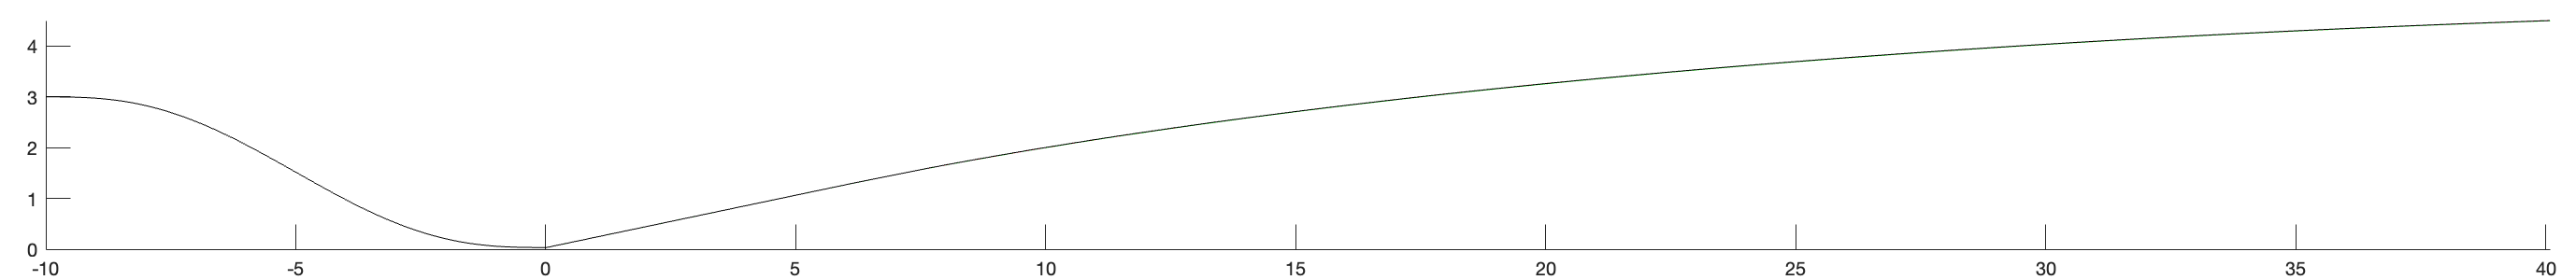
\includegraphics[width=6in]{contour}
    \caption{Final nozzle contour defined by analytic functions.}
    \label{fig:contour}
\end{figure}

\pagebreak
